\section{Semantic Relatedness Measurement}
\label{sr}
We give an overview of our model in figure \ref{overview} where solid lines lead the flow of model and dotted lines
demonstrate that there is an additional function from source part to target part. \
This figure illustrates the construction of our network and the relatedness measurement.
For the words in vocabulary, we can get a mapping between words and concepts(pages in Wikipedia)
by corpus statistics. Then we query the unique entity by the page id in DBPedia SPARQL endpoint.
For the layer of entity-to-entity, we divide it into attributes and topological structure and embed them by different models. 
As for the semantic relatedness computing, we consider three layers relatedness measurement:
word-to-word, word-to-entity and entity-to-entity when it comes to knowledge association network.

\begin{figure*}
    \flushleft
    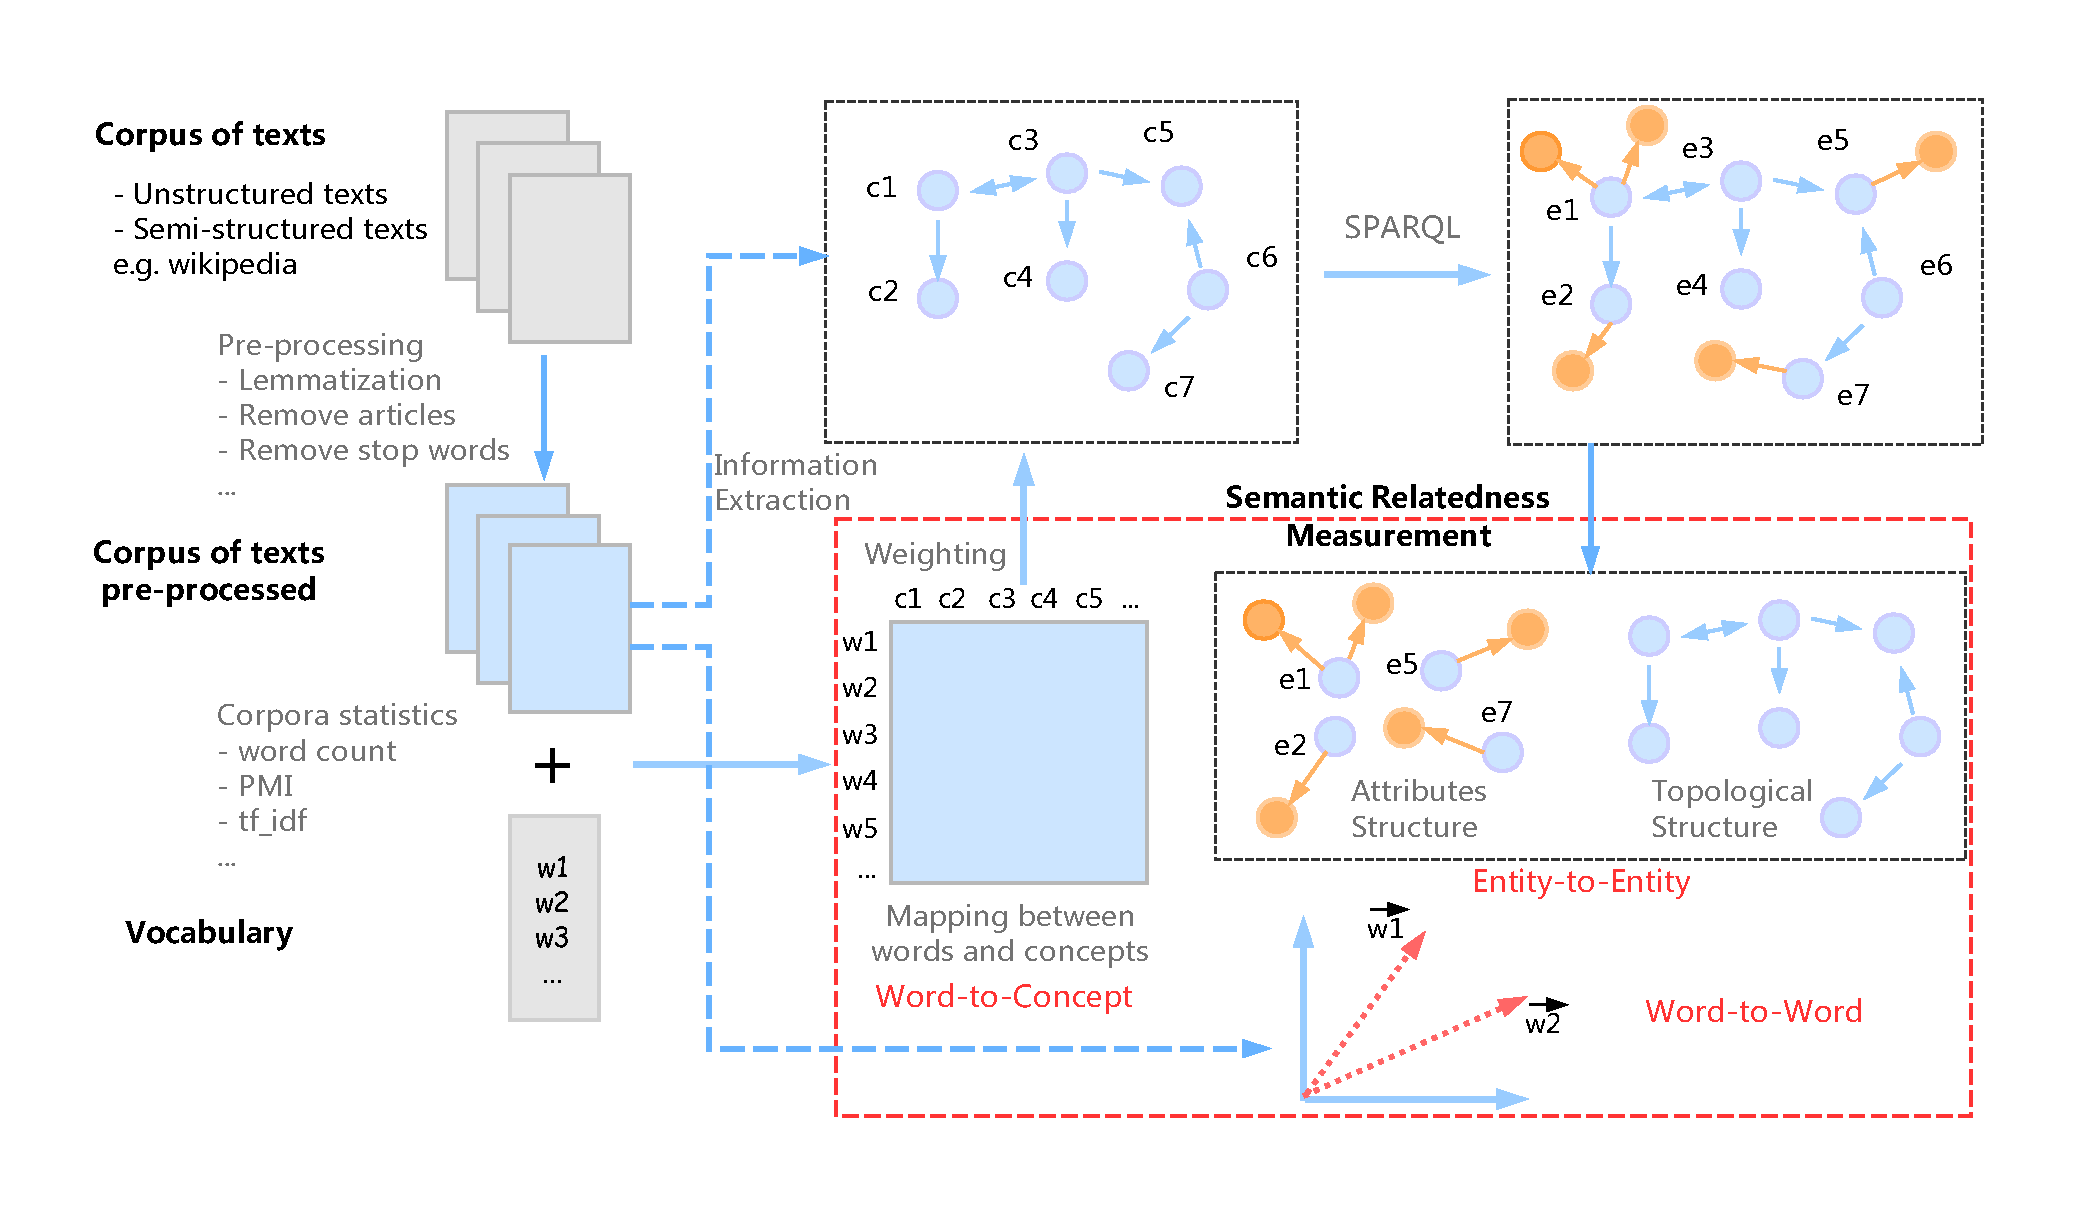
\includegraphics[width=1\textwidth]{pic/association-network.pdf}\\
    \caption{Association Network in Semantic measurement}
    \label{overview}
\end{figure*}

\subsection{word-to-word}
The semantic relatedness in word layer is mainly measured by 1) distributed vector representation such as word2vec \cite{corr/Mikolov13} 
and GloVe \cite{emnlp/PenningtonSM14} etc. 2) word co-occurrence, which means two words are relevant if they appear in a window size K. 
Experimental results prove that distributed vector representation works better in computing semantic relatedness\cite{corr/Mikolov13}.
Therefore in this paper, we abandon co-occurrence-based methods and adopt word2vec to train the Wikipedia corpus to product effective
vector representation for each word. 
Let $\overrightarrow v_i$ and $\overrightarrow v_j$ denote the vector representation of $w_i$ and $w_i$, and $f(w_i, w_j)$ is the semantic
relatedness score. The vector representation can be utilized to calculate the semantic relatedness based on cosine
function. Formally, we get:

\begin{small}
    \begin{equation}
        \label{cos}
        % \nonumber
        f_w(w_i, w_j) = cos(\overrightarrow v_i,\overrightarrow v_j) = \frac{\overrightarrow v_i \cdot 
        \overrightarrow v_j}{\left \| \overrightarrow v_i \right \|\left \| \overrightarrow v_j \right \|}
    \end{equation}
\end{small}

The word2vec algorithms include skip-gram and CBOW models, using either hierarchical softmax or negative sampling.
The combination of skip-gram and negative sampling are used frequently and effective experimentally. We choose this
training program accordingly. The detailed parameter setting can be seen in the part of experiment.

\subsection{word-to-entity}
In the knowledge association network, there is a one-to-many relationship between words and entities in DBPedia.
For a given word, several relevant entities will rise from our network due to the word ambiguity.
To measure the degree of association between word($w$) and entity($e$), 1) some researchers\cite{aaai/Pirro12}
take the co-occurrence times between $w$ and $c$ as the judgement of relatedness,
which is insensitive for some common words like \emph{this}, \emph{that} and so on. 
2) and some other related works\cite{aaai/GongXH18} consider $w$ and $e$ are closely related if $e$ is the
only semantic meaning for word $w$. They compute the degree of strong connections between only anchor words and
their out link concepts based on the follow equation:

\begin{small}
    \begin{equation}
        \label{lp_link}
        LP(w, c) = \sum_{P}^{ }\sum_{w \in S}^{ } \frac{\sum_{w{'} \in S}^{ }tf\_idf(w^{'},c)}
        {\sum_{c^{'} \in c(w)}^{ }\sum_{w^{'} \in S}^{ }tf\_idf(w{'}, c{'})}
    \end{equation}
\end{small}where $P$ indicates a wiki page, $S$ represents one sentence in a wikipage that contains the word $w$, and
$w^{'}$ means every contextual word in $S$. $c(w)$ is a set of concepts which are linked from anchor word $w$. This method
just considers anchor words and out link concepts, but ignores the relationship between current page and the anchor texts.

It is well known that tf-idf is a numerical statistic that is intended to reflect how important a word is to a document
in a collection or corpus. From our point of view, in order to measure the relatedness between words and entities,
we adopt tf-idf measurement. Specially, we evaluate the relationship of mapping from words to Wikipedia pages as:

\begin{small}
    \begin{equation}
        \label{tfidf}
        f_{we}(w_i, e_j) = \frac{tf\_idf(w_i,e_j)}{\sum_{e^{'} \in e(w)}^{ }tf\_idf(w_i,e^{'})}
    \end{equation}
\end{small}where $e(w)$ is the entities set that are associated with $w$, and the wikipage of $e^{'}$ contains the word $w$.

\subsection{entity-to-entity}
The knowledge association network in entity-to-entity level is fundamentally a multi-relational graph
where an entity is described by discrete attributes and topological structure collectively.
It is unreasonable to just consider either of the these information. Two entities may hold totally different
attributes but they appear in the same Wikipedia page and vice verse. 
The part of attributes holds the detailed semantic information such as person A is the friend of B,
person B is the member of organization C etc. The topological structure in entity-level reflects the co-occurrence
of entities. Things get quite different in representation of semantic in these two structure. 
Consequently, we adopt two different methods to obtain vector representation of the attributes and the topological structure.

\subsubsection{embedding for attributes}
The straightforward method to embed a set of attributes around an entity is \emph{one-hot}. Nevertheless, a surprisingly
high number of attributes in DBPedia brings a insoluble problem for \emph{one-hot} because of the excessive dimensions.
From our point of view, there exists a \emph{1-to-1} relationship between entities and their attributes, which is
interpreted as a translation operation on the low-dimension embeddings of entities\cite{nips/BordesUGWY13,corr/Ledell17}.
Suppose there are $\mathrm{N}$ different attributes in our network and the attributes space is denoted as
$\mathbb{R} ^ {|N| \times |d|}$, where $d$ the dimension of embedding for one attribute.
Inspired by the translation embeddings on knowledge graph, we combine the relationships and entities to minimize
a margin ranking loss over the attributes graph $G_{attr}$:

\begin{small}
    \begin{equation}
        \nonumber
        \label{starspace_formula}
        \mathcal{L} = \sum_{(a,b) \in G_{attr}^+}^{ } \sum_{b^- \in G_{attr}^-}^{ }[\ell + cos(a,b)-cos(a,b^-)]_+
    \end{equation}
\end{small}where $[x]_+=max(0, x)$, and $\ell$ is a margin hyperparameter. 

In our model, the input data $G_{attr}$ is a set of $(h, r, t)$ triples, consisting of a head entity $h$, 
a relation $r$ and a tail entity $t$. The positive entity pair (a,b) is sampled from
attributes network $G_{attr}$, and we select uniformly at random to get positive sample $G_{attr}^+$ in two strategies:
(i) $a$ consists of the bag of $h$ and $r$, while $b$ consists of only $t$; 
(ii) $a$ consists of $h$, $b$ consists of $r$ and $t$. 
Negative entities $b^-$ are sampled from the set of possible triples $G_{attr}^-$.  
We utilizes a $k$-negative sampling strategy\cite{corr/Mikolov13} to select $k$ negative pairs for each batch update.
The optimization of method inherits the strategy of stochastic gradient descent(SGD). Each SGD step is one
sampling from $G_{attr}^+$ in the outer sum.

As a result, we take the entities attributes graph $G_{attr}$ of $(h, r, t)$ triples as inputs to train the model.
For each entity and relation in graph $G_{attr}$, there is a fixed-length vector which can
then be used to compute semantic relatedness via cosine function.


\subsubsection{embedding for topological structure}
The connections among a great deal of entities include many semantic relations such as \emph{Apple\_Inc} is the
\emph{manufacturer} of \emph{IPod}, person \emph{A} is the \emph{wife} of \emph{person B} etc. Most of these
relations contain specific semantic knowledge, but there is a relation named \emph{WikiPageRedirectOf} which
connects two entities if one entity's anchor text description is mentioned in the corresponding Wikipedia page of the other.
We can get the topological structure $G_{t}$ among entities on account of this redirection relation.
When somebody browses a wikipage and he wants to check a few out links which
are contained in current page, the most related out link will appear in his mind firstly. This situation indicates that
the edges in $G_{t}$ have different transition probability, which is a probability graph model shown in figure \ref{two_graph}.

The most straightforward way to weight the edges is to consider the occurrence number of the anchor text in a wikipage.
We intergrate the anchor text as a single term $t_i$ for an entity $e_i$.
Let $cnt(e_i, e_j)$ denote the co-occurrence frequency of
the term $t_j$ of $e_j$ that appears in page of $e_i$. Formally, for an entity-to-entity weighted edge $<e_i, e_j>$, we have:

\begin{small}
    \begin{equation}
        \nonumber
        \label{cng_formula}
        W_{cnt}(e_i, e_j) = \frac{cnt(e_i, e_j)}{\sum_{e^{'} \in p_i}^{ }cnt(e_i, e^{'})}
    \end{equation}
\end{small}where $W_{cnt}(e_i, e_j)$ denotes the probability from $e_i$ to $e_j$. $p_i$ is the corresponding Wikipedia page of $e_i$,
and contains some anchor texts for each $e^{'}$ in $p_i$.
However, just consider anchor text frequency would give some general frequent terms high degree of relatedness.
Thus we adopt $tf\_idf$ instead of co-occurrence principle to weigh how important an entity(anchor text) is to
another(current page). There is:

\begin{small}
    \begin{equation}
        \nonumber
        \label{w_tf-idf_formula}
        W_{tf\_idf}(e_i, e_j) = \frac{tf\_idf(e_i, e_j)}{\sum_{e^{'} \in p_i}^{ }tf\_idf(e_i, e^{'})}
    \end{equation}
\end{small} Then we can get the transition probability from $e_i$ to $e_j$:

\begin{small}
    \begin{equation}
        \nonumber
        \label{pr_formula}
        \begin{cases}
            & \text  P(e_j|e_i) = W(e_i, e_j)\\
            & \text W \in (W_{cnt}, W_{tf\_idf})
        \end{cases}
    \end{equation}
\end{small} 

In consideration of topological structure, in network, some embedding methods\cite{kdd/Perozzi14,kdd/GroverL16} for nodes
are mainly inspired by Skip-gram model. They represent a network as a "document". The same
way as a document is an ordered sequence of words, one could sample sequences of nodes from the underlying network and turn
a network into an ordered sequence of nodes. In this paper, to get expressive vector representations for nodes, we follow Skip-gram model
to get network embedding. Our first priority is to determine the sampling strategy. One excellent work called \emph{node2vec}\cite{kdd/GroverL16}
proposes a flexible neighborhood sampling strategy which allows us to smoothly interpolate between BFS and DFS.
They propose a search bias we called $\mathrm{a}$:

\begin{small}
    \begin{equation}
        \mathrm{a}_{pq}(t,x) = 
        \left\{\begin{matrix} 1/p & if\ d_{tx}=0
        & \\ 1 & if\ d_{tx}=1
        & \\ 1/q & if\ d_{tx}=2
        \end{matrix}\right.
    \end{equation}
\end{small}It can be exhibited in the right of figure \ref{two_graph}, edge labels indicate search biases $\mathrm{a}$. Suppose we start a random walk
which traverses the edge $(\mathrm{t}, \mathrm{v})$, now we are in node $\mathrm{v}$ and next can walk to $(\mathrm{t}, x_1, x_2)$.
There are $d_{tt}=0$, $d_{tx_1}=2$ and $d_{tx_2}=2$, so we can get the result biases shown in figure \ref{two_graph}.
Note that if node $\mathrm{t}$ and $x_2$ are connected, bias from $\mathrm{v}$ to $x_2$ would be 1.

The node embedding is a maximum likelihood optimization problem following Skip-gram model which uses one
word to predict its context. Analogously, given a sequence of entities $(e_0, e_1, ..., e_i, ...e_l)$ sampled from the network $G_t$,
for an entity $e_i$, we utilize it to predict the neighborhood entities, which is to estimate the likelihood:

\begin{small}
    \begin{equation}
        Pr = ((e_0, e_1, ..., e_{i-1}, e_{i+1}, ..., e_l)|e_i)
    \end{equation}
\end{small}We define $N(e_i)$ as the context entities around the entity $e_i$, and we introduce a mapping function
$\Phi: e \in E \rightarrow \mathbb{R}^{\left | E \right | \times d}$ where E is not the edge set of $G_t$ but the 
entity set i.e. node set. $\Phi$ is represented as a $\left | E \right | \times d$ matrix of parameters which will be
trained to get. For each $e_i \in E$, we will get a $d$-dimension vector. There is the loss function to minimize:

\begin{small}
    \begin{equation}
        min\  -log Pr(N(e_i)|\Phi(e_i)) = -log\prod_{e^{'} \in N(e_i)}^{ }Pr(e^{'}|\Phi(e_i))
    \end{equation}
\end{small}For $e^{'} \in N(e_i)$, it have a symmetric effect with $e_i$ in feature space\cite{kdd/GroverL16}.
So we adopt the softmax function to normalize the likelihood probability:

\begin{small}
    \begin{equation}
        Pr(e^{'}|\Phi(e_i)) = \frac{exp(\Phi(e^{'})\cdot \Phi(e_i))}{\sum_{e_k \in E}^{ }exp(\Phi(e_k)\cdot \Phi(e_i))}
    \end{equation}
\end{small}Finally, We optimize  likelihood function (6) using SGD.

\begin{figure}
    \flushleft
    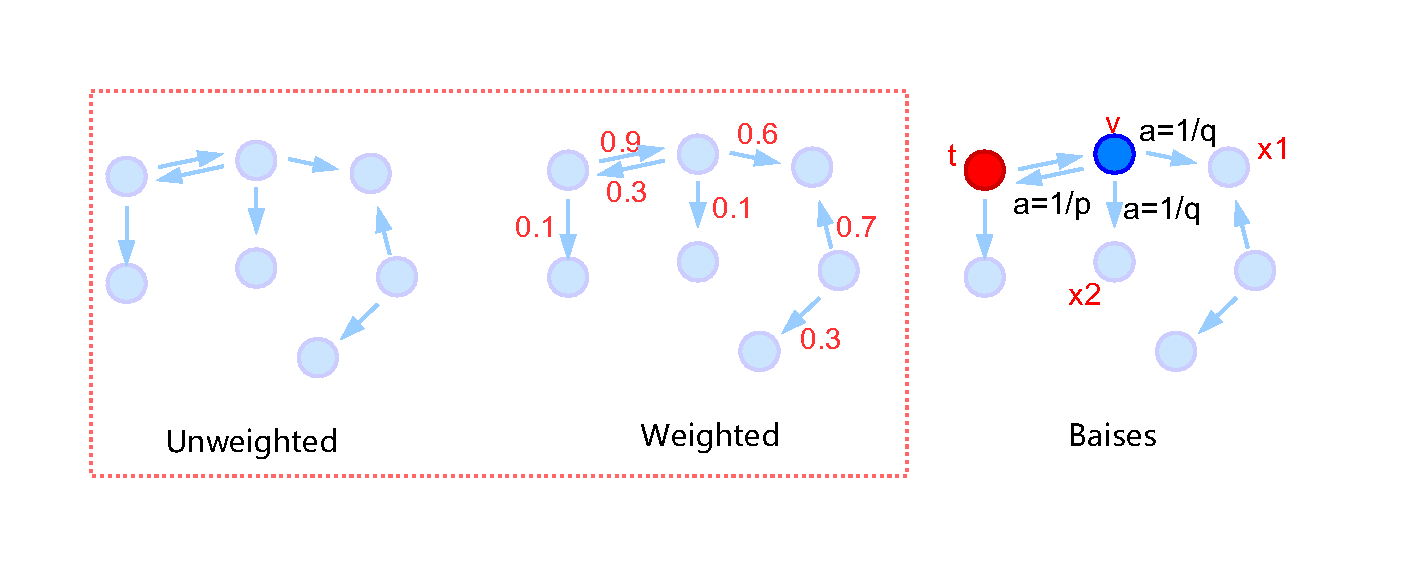
\includegraphics[width=0.5\textwidth]{pic/graph.pdf}\\
    \caption{Unweighted, Weighted topological structure and the random walk bias}
    \label{two_graph}
\end{figure}

\subsubsection{measurement}
We can get the embedding for an entity $e_i$, that consists of attributes information embedding($\overrightarrow {va}_i$) and
topological structure embedding($\overrightarrow {vt}_i$). Formally, we refer to the relatedness of entity-to-entity as:

\begin{small}
    \begin{equation}
        f_e(e_i, e_j) = \alpha cos({\overrightarrow {va}_i, \overrightarrow {va}_j}) 
        + (1-\alpha)cos(\overrightarrow {vt}_i,\overrightarrow {vt}_j)
    \end{equation}
\end{small}where $\alpha \in [0,1]$ is to adjust the weights of two parts.


\subsection{Word Semantic Relatedness \emph{F}}
We consider three layers for final semantic relatedness measurement including word-to-word, word-to-entity and entity-to-entity.
The word-to-entity and entity-to-entity are combined as concept-layer relatedness $F_c(w_i, w_j)$, and we refer to
word-to-word to word-layer relatedness named $F_w(w_i, w_j)$. Formally, We have:

\begin{small}
    \begin{equation}
        F_c(w_i, w_j) = \sum_{e_i \in E_i}^{ }\sum_{e_j \in E_j}^{ }f_{we}(w_i, e_i)f_e(e_i, e_j)f_{we}(w_j, e_j)
    \end{equation}
\end{small}in which $E_i$ is the entities set that is associated with word $w_i$.
The final word semantic relatedness measurement are:

\begin{small}
    \begin{equation}
        F(w_i, w_j) = \varphi F_w(w_i, w_j) + (1 - \varphi) F_c(w_i, w_j)
    \end{equation}
\end{small} $\varphi \in [0,1]$ trades off the weight of $F_w$ against $F_c$.




